%
% chapter.tex 
%
% (c) 2018 Prof Dr Andreas Müller, Hochschule Rapperswil
%
\chapter{Orthogonalität\label{chapter:orthogonalitaet}}
\lhead{Orthogonalität}
\rhead{}
In der bisher entwickelten Vektorgeometrie haben Längen und Winkel keine 
Rolle gespielt.
Wir haben akzeptiert, dass lineare Abbildungen aus der Elementargeometrie
bekannte Eigenschaften wie Rechtwinkligkeit von Geraden oder Gleichseitigkeit
von Dreiecken zerstören können.
Wir hatten keine Wahl, weil wir kein Werkzeug zur Verfügung hatten, 
um Längen und Winkel zu messen.
Das Skalarprodukt ist dieses zusätzliche Werkzeug, wir führen es in
Abschnitt~\ref{section:ortho-skalar} ein.

Mit dem Skalarprodukt eröffnet sich ein ganze Menge neuer Anwendungen.
Wir können Geraden und Ebenen jetzt noch etwas prägnanter mit
der Normalenform beschreiben (Abschnitt~\ref{section:normalform}),
wir können besonders gut geeignete Basen konstruieren, in denen die
Zerlegung in Komponenten speziell einfach ist
(Orthonormalbasis, Abschnitt~\ref{section:orthonormalbasis}),
wir können Kreise und Kugeln
beschreiben (Abschnitt~\ref{section:kreisundkugel}) und wir können eine
allgemeine Technik für die Lösung von überbestimmten Gleichungssystemen
entwickeln (Least Squares, Abschnitt~\ref{section:ueberbestimmt}).
In Abschnitt~\ref{section:orthabb} charakterisieren wir Abbildungen,
die das Skalarprodukt nicht verändern, sie beschreiben Bewegungen
des Raumes.

%\begin{verbatim}
5.1 Determinante und Orientierung
- Orientierter Flächeninhalt
- Orientiertes Volumen
5.2 Vektorprodukt
- Definition und Eigenschaften
- Normalenvektoren
- Abstandsformeln
\end{verbatim}



%
% skalar.tex -- Skalarprodukt
%
% (c) 2018 Prof Dr Andreas Müller, Hochschule Rapperswil
%
\section{Orthogonale Projektion und Skalarprodukt\label{section:ortho-skalar}}
\rhead{Orthogonale Projektion und Skalarprodukt}
\index{Skalarprodukt}
Abstand und Winkel spielen in der euklidischen Geometrie eine fundamentale
Rolle.
Die bisher eingeführten Elemente der Vektorgeometrie erlauben
jedoch noch nicht, Abstände oder Winkel zu berechnen.
Aus der elementaren Trigonometrie ist bekannt, dass der Schlüssel dazu
das Verständnis rechtwinkliger Dreiecke ist.
Der Kosinus eines Winkels ist das Verhältnis von Ankathete zu Hypothenuse.
De Ankathete ist aber auch die orthogonale Projektion der Hypothenuse
auf die Richtung der Ankathete.
Das Skalarprodukt soll daher aus der orthogonalen Projektion entwickelt
werden.

%
% Orthgonale Projektion
%
\subsection{Orthogonale Projektion\label{subsection:orthoproj}}
\index{orthogonale Projektion}
\index{Projektion!orthogonale|see{orthogonale Projektion}}
Zunächst möchten wir zeigen, dass sich Längen und Winkel berechnen
lassen, wenn man in der Lage ist, die Länge der orthogonalen Projektion
eines Vektors $\vec{v}$ auf jeden beliebigen anderen Vektor $\vec{u}$
zu berechnen.
\begin{figure}
\begin{center}
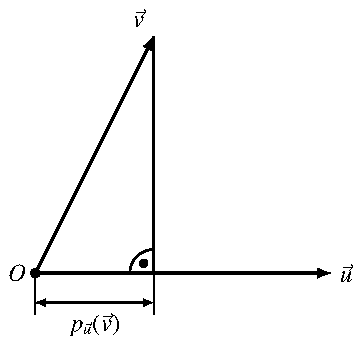
\includegraphics{4/images/projektion.pdf}
\end{center}
\caption{Orthogonale Projektion\label{orthproj}}
\end{figure}

Seien also $\vec u$, $\vec v$ zwei beliebige Vektoren wie in Abbildung~\ref{orthproj} und $p_{\vec u}(\vec v)$
die Länge der Projektion des Vektors $\vec v$ auf $\vec u$.
Wir versehen diese Länge mit einem Vorzeichen, zeigt der auf $\vec u$
projizierte Vektor $\vec v$ in die gleiche Richtung wie $\vec u$
nehmen wir die Länge positiv, zeigt der projizierte Vektor in die
Gegenrichtung, ist $p_{\vec u}(\vec v)$ negativ.

Die Länge von $\vec v$ ist $p_{\vec v}(\vec v)$, und für den Winkel
$\alpha$ zwischen den beiden Vektoren ist
\begin{equation}
\cos \alpha = \frac{p_{\vec u}(\vec v)}{p_{\vec v}(\vec v)}.
\label{zwischenwinkel}
\end{equation}
Offenbar ist die Länge der Projektion die grundlegendere Grösse,
aus der man die anderen Konzepte ableiten kann.
Etwas ungünstig ist an dieser Projektion nur, dass die beiden Vektoren nicht
symmetrisch eingehen.
\begin{figure}
\centering
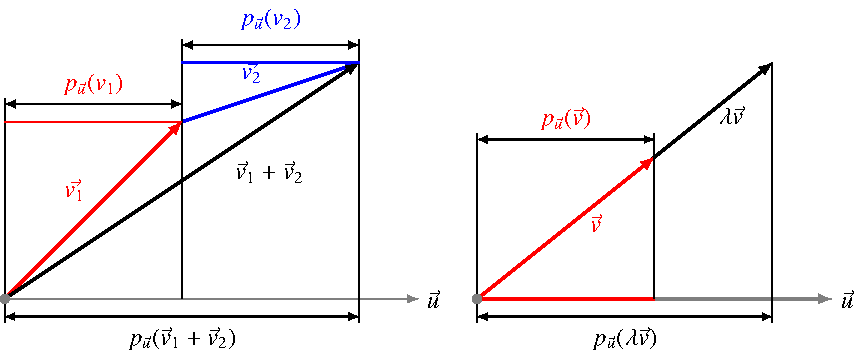
\includegraphics{4/images/linearitaet.pdf}
\caption{Die Projektionsabbilung
$\vec{v}\mapsto p_{\vec{u}}(\vec{v})$
ist linear. Die linke Graphik zeigt
$p_{\vec{u}}(\vec{v}_1+\vec{v}_2)
=
p_{\vec{u}}(\vec{v}_1)+p_{\vec{u}}(\vec{v}_2)$,
die rechte ist der Strahlensatz und zeigt
$p_{\vec{u}}(\lambda\vec{v})=\lambda p_{\vec{u}}(\vec{v})$.
\label{projektionlinearitaet}}
\end{figure}
Immerhin ist $p_{\vec u}(\vec v)$ linear in $\vec v$, wie man
sich mit der Abbildung~\ref{projektionlinearitaet}
sofort überzeugen kann, es ist also
\begin{align*}
p_{\vec u}(\vec v_1+\vec v_2)
&=
p_{\vec u}(\vec v_1)+p_{\vec u}(\vec v_2)
\\
p_{\vec u}(\lambda \vec v)
&=
\lambda p_{\vec u}(\vec v).
\end{align*}

%
% Skalarprodukt
%
\subsection{Skalarprodukt}
\index{Skalarprodukt}
\begin{figure}
\begin{center}
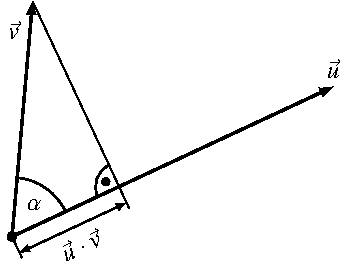
\includegraphics{4/images/skalarprodukt.pdf}
\end{center}
\caption{Skalarprodukt $\vec u\cdot \vec v$ des Einheitsvektors $\vec u$
und des Vektors $\vec v$ mit Zwischenwinkel
$\alpha$.\label{image-skalarprodukt}}
\end{figure}
Gesucht ist daher eine Konstruktion, welche immer noch linear ist,
aber auch symmetrisch in $\vec u$ und $\vec v$.
Die Formel (\ref{zwischenwinkel}) deutet auch an, wie dies erreicht
werden kann.
Der Zwischenwinkel kann natürlich auch berechnet werden,
indem die beiden Vektoren vertauscht werden:
\[
\cos \alpha
=
\frac{p_{\vec u}(\vec v)}{p_{\vec v}(\vec v)}
=
\frac{p_{\vec v}(\vec u)}{p_{\vec u}(\vec u)}
\]
Multipliziert man diese Gleichung mit
$
p_{\vec u}(\vec u)
p_{\vec v}(\vec v)
$, erhält man
\[
\vec u\cdot\vec v
=
p_{\vec u}(\vec u)
p_{\vec v}(\vec v)
\cos\alpha =
p_{\vec u}(\vec u)p_{\vec u}(\vec v)
=
p_{\vec v}(\vec v)p_{\vec v}(\vec u),
\]
was offenbar symmetrisch in $\vec u$ und $\vec v$ ist.

\begin{definition}Das Skalarprodukt zweier Vektoren $\vec u$ und
$\vec v$ ist
\[
\vec u\cdot\vec v
=
p_{\vec u}(\vec u)
p_{\vec v}(\vec v)
\cos\alpha.
\]
\end{definition}
Diese Grösse ist linear in $\vec u$ und linear in $\vec v$ und man kann
daraus $p_{\vec u}(\vec v)$ mittels
\[
p_{\vec u}(\vec v)
=
\frac{p_{\vec u}(\vec v)p_{\vec u}(\vec u)}{p_{\vec u}(\vec u)}
=
\frac{\vec u\cdot\vec v}{\sqrt{p_{\vec u}(\vec u)^2}}
=
\frac{\vec u\cdot\vec v}{\sqrt{\vec u\cdot \vec u}}
\]
wieder zurückgewinnen.

\begin{satz}
Seien $\vec u$ und $\vec v$ zwei Vektoren, dann ist
\[
|\vec u|=p_{\vec u}(\vec u)=\sqrt{\vec u\cdot\vec u}
\]
die Länge des Vektors und für den Zwischenwinkel $\alpha$ gilt
\[
|\vec u|\,|\vec v|\cos\alpha=\vec u\cdot\vec v.
\]
Zwei vom Nullvektor verschiedene Vektoren  stehen genau dann senkrecht
aufeinander, wenn $\vec u\cdot\vec v=0$.
%Die Projektion $\vec v_{\|}$ von $\vec v$ auf $\vec u$ ist
%\[
%\vec v_{\|}=\frac{\vec v\cdot\vec u}{\vec u\cdot\vec u}\vec u.
%\]
%Ist $\vec u$ ein Einheitsvektor, dann ist $\vec v_{\|}=(\vec v\cdot \vec u)\vec u$.
\end{satz}
\index{Zwischenwinkel}

%
% Skalarprodukt und Standardbasis
%
\subsection{Skalarprodukt und Standardbasis}
Zur praktischen Berechnung des Skalarproduktes benötigen wir
eine Formel, die das Skalarprodukt aus den Vektorkomponenten
berechnet.
Schreibt man
\[
\vec u=\begin{pmatrix}u_1\\u_2\\u_3\end{pmatrix}
=u_1\vec e_1+u_2\vec e_2+u_3\vec e_3
,
\qquad
\vec v=\begin{pmatrix}v_1\\v_2\\v_3\end{pmatrix}
=v_1\vec e_1+v_2\vec e_2+v_3\vec e_3
\]
dann kann das Skalarprodukt mit der Linearität berechnet werden:
\begin{align*}
\vec u\cdot\vec v
&=
(u_1\vec e_1+u_2\vec e_2+u_3\vec e_3)\cdot
(v_1\vec e_1+v_2\vec e_2+v_3\vec e_3)
\\
&=
u_1v_1\vec e_1\cdot\vec e_1+
u_1v_2\vec e_1\cdot\vec e_2+
u_1v_3\vec e_1\cdot\vec e_3\\
&\qquad +
u_2v_1\vec e_2\cdot\vec e_1+
u_2v_2\vec e_2\cdot\vec e_2+
u_2v_3\vec e_2\cdot\vec e_3\\
&\qquad+
u_3v_1\vec e_3\cdot\vec e_1+
u_3v_2\vec e_3\cdot\vec e_2+
u_3v_3\vec e_3\cdot\vec e_3
\end{align*}
Die Skalarprodukte von aufeinander senkrecht stehenden Vektoren
verschwinden.
Es bleiben nur die Termen mit $\vec e_i\cdot\vec e_i$.
Das Skalarprodukt eines Vektors mit sich selbst ist das Quadrat
der Länge, also $\vec e_i\cdot \vec e_i=1$ und so erhalten wir den
folgenden Satz.
\begin{satz}
Das Skalarprodukt zweier Vektoren
\[
\vec u=\begin{pmatrix}u_1\\u_2\\u_3\end{pmatrix},
\qquad
\vec v=\begin{pmatrix}v_1\\v_2\\v_3\end{pmatrix}
\]
ist
\[
\vec u\cdot\vec v
=
u_1v_1+u_2v_2+u_3v_3.
\]
\end{satz}

\begin{beispiel}
Berechne die Länge und den Zwischenwinkel der Vektoren
\begin{align*}
\vec a&= \begin{pmatrix} 3\\12\\ 4 \end{pmatrix},
&
\vec b&= \begin{pmatrix}2\\3\\6\end{pmatrix}.
\end{align*}

\smallskip

{\parindent 0pt Die} Länge der Vektoren ist
\begin{align*}
|\vec a|
&
=\sqrt{\vec a\cdot \vec a}
&
|\vec b|
&
=\sqrt{\vec b\cdot \vec b}
\\
&=\sqrt{9+144+16}
&
&=\sqrt{4+9+36}
\\
&=\sqrt{169}=13
&
&
=\sqrt{49}=7
\end{align*}
Damit kann man jetzt auch den Zwischenwinkel berechnen
\begin{align*}
\cos\alpha&= \frac{\vec a\cdot \vec b}{|\vec a|\;|\vec b|}
=
\frac{6+36+24}{13\cdot 7}=\frac{66}{91}=0.72527
\\
\alpha&=43.51^\circ
\end{align*}
\end{beispiel}
Häufig braucht man zu einem Vektor einen Vektor mit gleicher Richtung,
aber Einheitslänge.
Wir verwenden die Schreibweise
\[
\vec{v}^0 = \frac{\vec{v}}{|\vec{v}|}
\]
für den zum Vektor $\vec{v}$ gehörigen Einheitsvektor.


%
% anwendungen.tex -- Anwendungen des Skalarproduktes
%
% (c) 2018 Prof Dr Andreas Müller, Hochschule Rapperswil
%
\section{Erste Anwendungen des Skalarproduktes\label{section:normalform}}
\rhead{Erste Anwendungen des Skalarproduktes}
Aus den Eigenschaften des Skalarproduktes ergeben sich unmittelbar
erste Anwendungen.

%
% Normalenform von Ebene und Gerade
%
\subsection{Normalenform von Ebene und Gerade}
\begin{figure}
\begin{center}
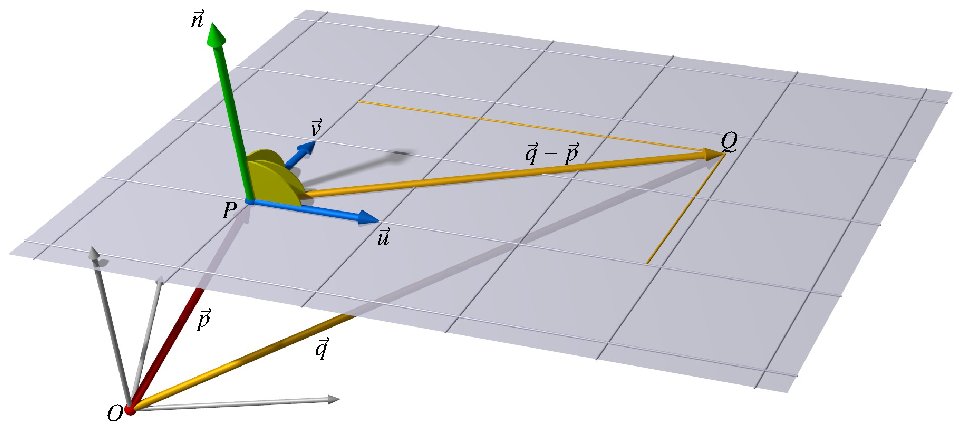
\includegraphics{4/images/normalenform.pdf}
\end{center}
\caption{Ebene in Normalenform\label{image-normalenform}}
\end{figure}
Das Skalarprodukt gibt uns eine neue Möglichkeit, Ebenen zu
beschreiben.
Eine Ebene durch den Punkt $P$ senkrecht auf den Vektor
$\vec n$ besteht genau aus jenen Punkten $Q$, für die der Vektor
$\overset{\rightarrow}{PQ}$ auf $\vec n$ senkrecht steht
(Abbildung~\ref{image-normalenform}).
Mit dem Skalarprodukt
ausgedrückt: Die Menge der Ortsvektoren der Punkte einer Ebene durch $P$ mit
\index{Normale}
Normale $\vec n$ ist
\[
\{\vec r\;|\;(\vec r-\vec p)\cdot \vec n=0\}
\]
Multipliziert man die Gleichung aus, erhält man
\begin{align*}
\left(
\begin{pmatrix}x\\y\\z\end{pmatrix}
-\begin{pmatrix}p_1\\p_2\\p_3\end{pmatrix}\right)\cdot
\begin{pmatrix}n_1\\n_2\\n_3\end{pmatrix}&=0
\\
(x-p_1)n_1+(y-p_2)n_2+(z-p_3)n_3&=0
\\
n_1x+n_2y+n_3z&=p_1n_1+p_2n_2+p_3n_3
\end{align*}
Diese Form der Ebenengleichung, in der $\vec n$ ein Einheitsnormalenvektor ist,
heisst auch {\em Hessesche Normalform}.
\index{Normalenform}
\index{Hessesche Normalform}

\begin{satz}
Ist $\vec n$ ein Einheitsvektor, dann ist
\[
d=(\vec r-\vec p_0)\cdot \vec n
\]
der Abstand des Punktes mit dem Ortsvektor $\vec r$ von der Ebene durch
den Punkt mit Ortsvektor $\vec p_0$ und Normalen $\vec n$.
In Koordinaten:
\[
d=n_xx+n_yy+n_zz-\vec p_0\cdot\vec n
\]
\end{satz}
\begin{proof}[Beweis]
$(\vec r-\vec p)\cdot \vec n$ ist die Länge der Projektion des Vektors
$\vec r -\vec p$ auf den Normalenvektor $\vec n$, also genau der behauptete
Abstand.
\end{proof}

\begin{beispiel}
Man finde die Normalenform der Ebenengleichung (\ref{beispielebene}) auf
Seite~\pageref{beispielebene},
und berechne den Abstand des Punktes $(1,1,1)$ von der Ebene.

\medskip

{\parindent 0pt Die} Lösung vollzieht sich in folgenden Schritten:
\begin{compactenum}
\item Bestimme die Normale der Ebene.
\item Schreibe die Gleichung der Ebene in Normalenform.
\item Bringe die Normalenform in Hessesche Normalform.
\item Berechne den Abstand des Punktes $(1,1,1)$.
\end{compactenum}
Gesucht ist ein Vektor $\vec n$, der auf beiden
Richtungsvektoren senkrecht steht, also
\begin{equation}
\begin{pmatrix}n_1\\n_2\\n_3\end{pmatrix}
\cdot
\begin{pmatrix}2\\2\\-2\end{pmatrix}
=0,
\qquad
\begin{pmatrix}n_1\\n_2\\n_3\end{pmatrix}
\cdot
\begin{pmatrix}3\\-3\\-1\end{pmatrix}
=0
\label{gleichungen-fuer-normale}
\end{equation}
Dies ist gleichbedeutend mit dem Gleichungssystem
\[
\begin{pmatrix}
2&2&-2\\
3&-3&-1
\end{pmatrix}
\begin{pmatrix}n_1\\n_2\\n_3\end{pmatrix}
=\begin{pmatrix}0\\0 \end{pmatrix}
\]
Der Gauss-Algorithmus liefert
\begin{align*}
\begin{tabular}{|>{$}c<{$}>{$}c<{$}>{$}c<{$}|}
\hline
2%
\begin{picture}(0,0)
\color{red}\put(-3,4){\circle{12}}
\end{picture}%
&2&-2\\
3%
\begin{picture}(0,0)%
\color{blue}\drawline(-8,-2)(-8,10)(2,10)(2,-2)
\end{picture}%
&-3&-1\\
\hline
\end{tabular}
&\rightarrow
\begin{tabular}{|>{$}c<{$}>{$}c<{$}>{$}c<{$}|}
\hline
1&1&-1\\
0&-6%
\begin{picture}(0,0)%
\color{red}\put(-7,4){\circle{15}}
\end{picture}%
&2\\
\hline
\end{tabular}
\rightarrow
\begin{tabular}{|>{$}c<{$}>{$}c<{$}>{$}c<{$}|}
\hline
1&1%
\begin{picture}(0,0)
\color{blue}\drawline(-8,10)(-8,-2)(2,-2)(2,10)
\end{picture}%
&-1\\
0&1&-\frac13\\
\hline
\end{tabular}
\rightarrow
\begin{tabular}{|>{$}c<{$}>{$}c<{$}>{$}c<{$}|}
\hline
1&0&-\frac23\\
0&1&-\frac13\\
\hline
\end{tabular}
\end{align*}
Die Komponente $n_3$ ist frei wählbar, wir setzen $n_3=3$, und bekommen
$n_1=2$ und $n_2=1$.
Tatsächlich ist
\begin{align*}
\begin{pmatrix}2\\1\\3\end{pmatrix}
\cdot
\begin{pmatrix}2\\2\\-2\end{pmatrix}
&=4+2-6=0
&
\begin{pmatrix}2\\1\\3\end{pmatrix}
\cdot
\begin{pmatrix}3\\-3\\-1\end{pmatrix}
&=6-3-3=0.
\end{align*}
Damit ist die Normalenform der Ebenengleichung
\begin{align}
\begin{pmatrix}2\\1\\3\end{pmatrix}\cdot\left(
\begin{pmatrix}x\\y\\z\end{pmatrix} - \begin{pmatrix}1\\2\\1\end{pmatrix}
\right)&=0\notag\\
\Rightarrow\qquad
2x+y+3z&=7\label{normalenform}
\end{align}
Diese Form ist zwar eine Normalenform, aber noch nicht die Hessesche
Normalform, da man für diesen Zweck einen Einheitsvektor als
Normalenvektor verwenden muss.
Unser Normalenvektor hat aber die Länge $|\vec n|=\sqrt{14}$.
Dividieren wir die Gleichung (\ref{normalenform})
durch $\sqrt{14}$, erhalten wir die Hessesche Normalform:
\begin{equation}
d=\frac{2}{\sqrt{14}}x+\frac{1}{\sqrt{14}}y+\frac{3}{\sqrt{14}}z-\frac{7}{\sqrt{14}}.
\label{hnf}
\end{equation}
Die Hessesche Normalform berechnet den Abstand eines Punktes von der
Ebene.
Man muss jetzt also nur noch den Punkt $(1,1,1)$ in die  Gleichung
(\ref{hnf}) einsetzen:
\[
d = (2+1+3-7)/\sqrt{14}=-1/\sqrt{14}=-0.26726,
\]
der gesuchte Abstand ist also $d=0.26726$.
\end{beispiel}

%
% Spiegelungen an einer Geraden oder Ebenen
%
\subsection{Spiegelung an einer Geraden oder Ebenen\label{spiegelung}}
\begin{figure}
\begin{center}
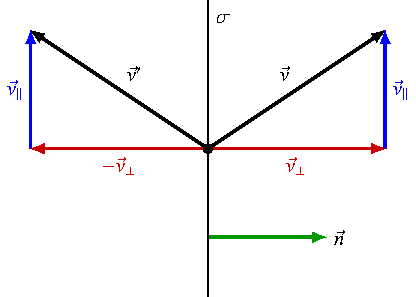
\includegraphics{4/images/spiegelung.pdf}
\end{center}
\caption{Spiegelung eines Vektors $\vec v$ an der Ebene senkrecht auf $\vec n$.
\label{image-spiegelung}}
\end{figure}
Da man mit dem Skalarprodukt senkrechte Projektionen berechnen kann,
muss es auch möglich sein, die Spiegelung eines Vektors $\vec v$
an einer Ebene mit Normale $\vec n$ zu berechnen ($|\vec n|=1$).
Dazu zerlegt man den Vektor $\vec v$ in eine Komponente $\vec v_{\|}$
parallel zur Ebene und eine Komponenten $\vec v_{\perp}$ senkrecht dazu,
also $\vec v=\vec v_{\|}+\vec v_{\perp}$ (Abbildung~\ref{image-spiegelung}).
Die senkrechte Komponente
ist im wesentlichen die Projektion von $\vec v$ auf $\vec n$:
\[
\vec v_{\perp}=
(\vec v\cdot\vec n)\vec n
.
\]
Die parallele Komponente ist der Rest:
\[
\vec v_{\|}=\vec v -\vec v_{\perp}=
\vec v-(\vec v\cdot\vec n)\vec n
,
\]
Beim gespiegelten Vektor zeigt die senkrechte Komponente in die
entgegengesetzte Richtung:
\begin{equation}
\vec v_{\text{gespiegelt}}=
\vec v_{\|}-\vec v_{\perp}
=
\vec v-(\vec v\cdot\vec n)\vec n
-
(\vec v\cdot\vec n)\vec n
=\vec v-2(\vec v\cdot\vec n)\vec n.
\label{equation:spiegelung}
\end{equation}

\begin{beispiel}
Man spiegle den Vektor $\vec a$ an der Ebene mit der Normalen $\vec n$,
\[
\vec a=\begin{pmatrix}1\\2\\3\end{pmatrix},
\qquad
\vec n=\begin{pmatrix}1\\1\\1\end{pmatrix}
\]

\smallskip

{\parindent 0pt Zunächst stellen wir fest,} dass $\vec n$ noch
kein Einheitsvektor ist, dass wir stattdessen $\vec n_0=\vec n/\sqrt{3}$
verwenden müssen.
Damit kann $\vec a$ jetzt die parallelen und orthogonalen
Komponenten zerlegt werden:
\[
\vec a_{\perp}=(\vec a\cdot\vec n_0)\vec n_0
=\frac1{\sqrt{3}} (1+2+3)\frac1{\sqrt{3}}\begin{pmatrix}1\\1\\1\end{pmatrix}
=\begin{pmatrix}2\\2\\2\end{pmatrix},
\quad
\vec a_{\|}=\begin{pmatrix} -1\\0\\1 \end{pmatrix}.
\]
Nach Formel (\ref{equation:spiegelung}) ist
\[
\vec a'=\vec a_{\|}-\vec a_{\perp}
=
\begin{pmatrix}-1\\0\\1\end{pmatrix}-\begin{pmatrix}2\\2\\2\end{pmatrix}
=\begin{pmatrix}-3\\-2\\-1\end{pmatrix}.
\]
der gespiegelt Vektor.
\end{beispiel}


%
% orthonrmalbasis.tex -- Orthonormierte Basis und Gram Schmidt
%
% (c) 2018 Prof Dr Andreas Müller, Hochschule Rapperswil
%
\section{Skalarprodukt und Basis\label{section:orthonormalbasis}}
\rhead{Skalarprodukt und Basis}
Bei der Berechnung des Skalarproduktes in Komponenten in der Standardbasis
hat sich gezeigt, dass eine Basis aus Einheitsvektoren, die zusätzlich
aufeinander senkrecht stehen, besonders gut für die Arbeit mit dem
Skalarprodukt geeignet ist.
Nicht immer hat man allerdings eine solch bequeme Basis.
In diesemAbschnitt sollen die Vorzüge einer solchen Basis nochmals
herausgearbeitet werden und es soll gezeigt werden, wie man aus
einer beliebigen Basis immer eine passende Basis aus orthogonalen
Einheitsvektoren machen kann.
Schliesslich wird gezeigt, wie sich das Skalarprodukt in einer beliebigen
Basis schreiben lässt.

%
% Orthonormalbasis
%
\subsection{Orthonormalbasis}
Die Vektoren $\vec e_i$ stehen senkrecht aufeinander und haben
Länge $1$.
Der Vektor
\[
\vec v
=
\begin{pmatrix}v_1\\v_2\\v_3\end{pmatrix}
\]
lässt sich mit Hilfe des Skalarproduktes als Summe von Vielfachen
der Vektoren $\vec e_i$ schreiben.
Es ist nämlich $v_i=\vec v\cdot\vec e_i$, also
\[
\vec v
=
\begin{pmatrix}v_1\\v_2\\v_3\end{pmatrix}
=
v_1\vec e_1
+
v_2\vec e_2
+
v_3\vec e_3
=
(\vec v\cdot \vec e_1)\vec e_1
+
(\vec v\cdot \vec e_2)\vec e_2
+
(\vec v\cdot \vec e_3)\vec e_3.
\]
Dies funktioniert aber nicht nur für die Vektoren $\vec e_i$.
Seien $\vec b_1$, $\vec b_2$ und $\vec b_3$ drei aufeinander senkrecht
stehende Vektoren der Länge $1$.
Mit dem Skalarprodukt kann man dies durch
\[
\vec b_i\cdot\vec b_j=\begin{cases}
0&\qquad i\ne j\\
1&\qquad i=j
\end{cases}
\]
ausdrücken.
Nun versucht man den Vektor $\vec v$ als Linearkombination
der Vektoren $\vec b_i$ zu schreiben, also als
\[
\vec v
=
v_1'\vec b_1
+
v_2'\vec b_2
+
v_3'\vec b_3.
\]
Multipliziert man jetzt beide Seiten dieser Gleichung mit $\vec{b}_i$,
erhält man
\begin{align*}
\vec v\cdot \vec b_i
&=
(
v_1'\vec b_1
+
v_2'\vec b_2
+
v_3'\vec b_3
)\cdot
\vec b_i
\\
&=
v_1'\vec b_1\cdot\vec b_i
+
v_2'\vec b_2\cdot\vec b_i
+
v_3'\vec b_3\cdot\vec b_i
\\
&=v_i',
\end{align*}
weil die Skalarprodukte $\vec{b}_j\cdot\vec{b}_i$ verschwinden für $i\ne j$
und $\vec{b}_i\cdot\vec{b}_i=1$.
Die Koordinaten $v_i'$ können also ganz einfach als Skalarprodukte 
$\vec{v}\cdot\vec{b}_i$ berechnet werden, wenn die Basis orthonormiert ist.

\begin{definition} Die Koeffizienten der Einheitsmatrix
\[
\delta_{ij}=
\begin{cases}
0&\qquad i\ne j\\
1&\qquad i=j
\end{cases}
\]
heissen {\em Kronecker-Delta}.
\end{definition}

\begin{definition}
$n$ Vektoren $\vec b_i$ heissen orthonormiert, wenn gilt
\[
\vec b_i\cdot\vec b_j=\delta_{ij}.
\]
\end{definition}

\begin{satz}
Sind die Vektoren $\vec b_i$ orthonormiert, dann kann man jeden
Vektor $\vec v$ als Linearkombination der Vektoren $\vec b_i$ schreiben:
\[
\vec v=
(\vec v\cdot\vec b_1)\vec b_1
+
(\vec v\cdot\vec b_2)\vec b_2
+
(\vec v\cdot\vec b_3)\vec b_3.
\]
Diese Darstellung ist eindeutig.
\end{satz}

\begin{proof}[Beweis]
Es ist nur noch zu beweisen, dass es nur eine solche Darstellung als
Linearkombination gibt.
Gäbe es zwei Darstellungen, also
\begin{align*}
\vec v
&=
v_1'\vec b_1+
v_2'\vec b_2+
v_3'\vec b_3\\
\text{und}\quad
\vec v
&=
v_1''\vec b_1+
v_2''\vec b_2+
v_3''\vec b_3,
\end{align*}
könnten wir die Differenz bilden:
\[
0=
(v_1'-v_1'')\vec b_1
+
(v_2'-v_2'')\vec b_2
+
(v_3'-v_3'')\vec b_3
\]
Multiplizieren wir diese Gleichung wieder mit $\vec{b}_i$, ergibt sich
\begin{align*}
0
&=
(v_1'-v_1'')\vec{b}_1\cdot\vec{b}_i
+
(v_2'-v_2'')\vec{b}_2\cdot\vec{b}_i
+
(v_3'-v_3'')\vec{b}_3\cdot\vec{b}_i
\\
\Rightarrow
\quad
0
&=
(v_i'-v_i'')
\\
\Rightarrow\quad
v_i'&=v_i''.
\end{align*}
Dies muss für jedes $i$ gelten, so dass alle
Koeffizienten $v_i'$ und $v_i''$ übereinstimmen.
\end{proof}

%
% Orthonormalisierung 
%
\subsection{Orthonormalisierung}
Für orthonormierte Vektoren ist es besonders einfach, eine Darstellung
eines beliebigen Vektors als Linearkombination zu finden.
Es ist daher sicher nützlich, aus einer Menge von Vektoren
$\{\vec a_1,\vec a_2,\vec a_3\}$
eine neue Menge von Vektoren zu konstruieren, die sich von der gegeben
möglichst wenig
unterscheidet, aber dennoch aus orthonormierten Vektoren besteht.

\begin{satz}[Gram-Schmidt]
\label{satz-gram-schmidt}
Seien $\{\vec a_1,\vec a_2,\vec a_3\}$ linear unabhängige Vektoren.
Dann gibt es orthonormierte Vektoren $\{\vec b_1,\vec b_2,\vec b_3\}$ so,
dass $b_k$ aus $a_1,\dots,a_k$ linear kombiniert werden kann, für jedes $k$.
Die $b_i$ lassen sich wie folgt berechnen
\begin{align*}
\vec b_1&=\frac1{|\vec a_1|}a_1\\
\vec b_2&=
\frac{
\vec a_2-(\vec a_2\cdot \vec b_1)\vec b_1
}{
|\vec a_2-(\vec a_2\cdot \vec b_1)\vec b_1|
}
\\
\vec b_3
&=
\frac{
\vec a_3-(\vec a_3\cdot \vec b_1)\vec b_1-(\vec a_3\cdot\vec b_2)\vec b_2
}{
|
\vec a_3-(\vec a_3\cdot \vec b_1)\vec b_1-(\vec a_3\cdot\vec b_2)\vec b_2
|
}
\\
&\phantom{=}\vdots\\
\vec b_k&=\frac{\vec a_k-(\vec a_k\cdot \vec b_1)\vec b_1-(\vec a_k\cdot \vec b_2)\vec b_2-\dots-(\vec a_k\cdot \vec b_{k-1})\vec b_{k-1}}{|\vec a_k-(\vec a_k\cdot \vec b_1)\vec b_1-(\vec a_k\cdot \vec b_2)\vec b_2-\dots-(\vec a_k\cdot \vec b_{k-1})\vec b_{k-1}|}
\end{align*}
Das Verfahren lässt sich offenbar auf eine beliebige Zahl linear
unabhängiger $n$-dimensionaler Vektoren verallgemeinern.
\end{satz}

Auf die Reihenfolge der Vektoren kommt es entscheidend an, wie die
folgenden zwei Beispiele zeigen
\begin{beispiel}
Die Vektoren
\[
\vec a_1=\begin{pmatrix}1\\0\\0\end{pmatrix},\qquad
\vec a_2=\begin{pmatrix}1\\1\\0\end{pmatrix},\qquad
\vec a_3=\begin{pmatrix}1\\1\\1\end{pmatrix}
\]
sind zu orthonormieren.

Die Formeln aus Satz~\ref{satz-gram-schmidt} liefern folgende Vektoren:
\begin{align*}
\vec b_1&=\frac{\vec a_1}{|\vec a_1|}=\begin{pmatrix}1\\0\\0\end{pmatrix}\\
\vec b_2&=
\frac{
\vec a_2-(\vec a_2\cdot \vec b_1)\vec b_1
}{
|\vec a_2-(\vec a_2\cdot \vec b_1)\vec b_1|
}
=
\frac{
\begin{pmatrix}1\\1\\0\end{pmatrix}-1\cdot\begin{pmatrix}1\\0\\0\end{pmatrix}
}{\dots}=\begin{pmatrix}0\\1\\0\end{pmatrix}\\
\\
\vec b_3&=
\frac{\vec a_3 -(\vec a_3\cdot \vec b_1)\vec b_1-(\vec a_3\cdot\vec b_2)\vec b_2}{\dots}
=\frac{\begin{pmatrix}1\\1\\1\end{pmatrix}-1\cdot \begin{pmatrix}1\\0\\0\end{pmatrix}-1\cdot\begin{pmatrix}0\\1\\0\end{pmatrix}
}{\dots}=\begin{pmatrix}0\\0\\1\end{pmatrix}
\end{align*}
Man findet also genau die Vektoren der Standardbasis.
\end{beispiel}

\begin{beispiel}
Die Vektoren
\[
\vec a_1=\begin{pmatrix}1\\0\\0\end{pmatrix},\qquad
\vec a_2=\begin{pmatrix}1\\1\\1\end{pmatrix},\qquad
\vec a_3=\begin{pmatrix}1\\1\\0\end{pmatrix}
\]
sind zu orthonormieren.

Dieses Beispiel unterscheidet sich vom vorangegangenen nur
durch die Reihenfolge der Vektoren.
Wieder können die Formeln von Satz~\ref{satz-gram-schmidt} angewandt werden:
\begin{align*}
\vec b_1&=\frac{\vec a_1}{|\vec a_1|}=\begin{pmatrix}1\\0\\0\end{pmatrix}
\\
\vec b_2
&=
\frac{\vec a_2-(\vec a_2\cdot \vec b_1)\vec b_1}{\dots}
=
\frac{\begin{pmatrix}1\\1\\1\end{pmatrix}-1\cdot\begin{pmatrix}1\\0\\0\end{pmatrix}}{\dots}=\frac1{\sqrt{2}}\begin{pmatrix}0\\1\\1\end{pmatrix}
\\
\vec b_3
&=
\frac{\vec a_3-(\vec a_3\cdot\vec b_1)\vec b_1-(\vec a_3\cdot\vec b_2)\vec b_2}{\dots}
=\frac{\displaystyle\begin{pmatrix}1\\1\\0\end{pmatrix}-1\cdot\begin{pmatrix}1\\0\\0\end{pmatrix}-\frac1{\sqrt{2}}\cdot\frac1{\sqrt{2}}\begin{pmatrix}0\\1\\1\end{pmatrix} }{\cdots}
=\frac{1}{\sqrt{2}}\begin{pmatrix}0\\1\\-1\end{pmatrix}.
\end{align*}
Die gefundenen Vektoren sind völlig verschiedenen von den Vektoren
im vorangegangenen Beispiel.
\end{beispiel}

%
% Skalarprodukt und Matrixprodukt
%
\subsection{Skalarprodukte und Matrixprodukt}
Das in der Vektorgeometrie definierte Skalarprodukt kann in beliebig
vielen Dimensionen definiert werden.
Zwei Vektoren $v$ und $u$ in $\mathbb R^n$ haben
das Skalarprodukt
\[
u\cdot v=
\begin{pmatrix}u_1\\\vdots\\u_n\end{pmatrix}
\cdot
\begin{pmatrix}v_1\\\vdots\\v_n\end{pmatrix}
=u_1v_1+\dots+u_nv_n=u^tv.
\]
Alle bisher entwickelten Anwendungen des Skalarproduktes lassen sich sofort
auf den $n$-di\-men\-sio\-nalen Raum übertragen.
Zum Beispiel ist die Länge eines Vektors definiert als
\[
|v|=\sqrt{v^tv}.
\]
Programme wie Octave oder Matlab brauchen daher keine spezielle Notation
für das Skalarprodukt, da mit Transposition und Matrixprodukt
bereits alles vorhanden ist, um das Skalarprodukt auszurechnen.
das Skalarprodukt der Spaltenvektoren
\texttt{u}
und
\texttt{v}
ist in Matlab-Notation
\texttt{u'*v}.

In den Anwendungen findet man aber weitere Beispiel von
Skalarprodukt-ähnlichen Grössen, zum Beispiel das Trägheitsmoment.
Die Rotationsenergie eines starren Körpers kann aus dem Vektor $\omega$
der Winkelgeschwindigkeit mit der (symmetrischen) Matrix des
Trägheitsmomentes $\Theta$
berechnet werden:
$
E=\frac12 \omega^t\Theta \omega.
$
Die allgemeinste Form eines Skalarproduktes verwendet daher eine
symmetrische Matrix $M$, also eine Matrix mit der Eigenschaft
$M=M^t$, und berechnet das Skalarprodukt zweier Vektoren $u$ und $v$
als $u^tMv$.
\begin{definition}
Ist $M$ eine symmetrische $n\times n$-Matrix, dann ist
\[
u^t Mv
=
\langle u,v\rangle_M
=
\langle u,v\rangle
\]
das zugehörige verallgemeinerte Skalarprodukt.
\end{definition}
Das gewöhnliche Skalarprodukt ist in dieser allgemeinen Definition
als der Fall $M=E$ enthalten.
Die Matrix
\[
M=\begin{pmatrix}
1& 0& 0& 0\\
0&-1& 0& 0\\
0& 0&-1& 0\\
0& 0& 0&-1
\end{pmatrix}
\]
führt auf das sogenannte Minkowski-Skalarprodukt, so benannt nach
Hermann Minkowski, der ab 1896 Professor an der ETH war und bei dem
Einstein studiert hat.
Es erlangt in der speziellen und allgemeinen Relativitätstheorie von
Einstein fundamentale Bedeutung.

%
% Basiswechsel
%
\subsection{Basiswechsel}
Sei wieder $T$ die Matrix, die Koordinaten $x$ von der Basis $B$ in die
Koordinaten $y$ in der Basis $B'$ umrechnet, also $y=Tx$.
Um das Skalarprodukt bezüglich der Basis $B'$ zu berechnen,
müssen die Vektoren zuerst mit $T^{-1}$ in die Basis $B$ umgerechnet werden,
so dass dann die Formel für das Skalarprodukt in der Basis $B$
verwendet werden kann:
\[
T^{-1}y\cdot T^{-1}\bar y
=
(T^{-1}y)^tT^{-1}\bar y
=
y^t (T^{-1})^tT^{-1} \bar y
\]
Die Matrix $(T^{-1})^tT^{-1}$ ist symmetrisch, der
``Spezialfall'' eines Skalarproduktes,
welches mit Hilfe einer symmetrischen Matrix definiert worden ist,
ist also unvermeidlich, wenn man die Basis wechseln will.


%
% kreis.tex 
%
% (c) 2018 Prof Dr Andreas Müller, Hochschule Rapperswil
%
\section{Kreis und Kugel\label{section:kreisundkugel}}
\rhead{Kreis und Kugel}
Da das Skalarprodukt die Länge eines Vektors berechnet, kann man
jetzt auch die Menge der Punkte eines Kreises in der Ebene
oder einer Kugel im Raum vektoriell beschreiben, und damit Standardaufgaben
lösen.

%
% Gleichungen von Kreis und Kugel
%
\subsection{Gleichungen von Kreis und Kugel}
\index{Kreis}
\index{Kugel}
Die Kugel $K(M,r)$ ist die Menge aller Punkte, die von einem festen Punkt, dem
Mittelpunkt oder Zentrum, alle den gleichen Abstand $r$ haben.
In vektorieller
Form heisst dies, dass die Ortsvektoren von Punkten mit dem Ortsvektor des
Mittelpunktes eine Differenz konstanter Länge haben.
Schreiben wir $\vec m$
für den Ortsvektor des Mittelpunktes, dann besteht die Kugel aus den
Punkten mit den Ortsvektoren
\[
K(M,r)
=
\{\vec p\;| \;|\vec p-\vec m|=r\}
=
\{\vec p\;| \;(\vec p-\vec m)\cdot(\vec p-\vec m)=r^2\}.
\]
Die zweite Form ist für die Lösung konkreter Problem oft nützlicher.

%
% Durchstosspunkt einer Geraden mit einer Kugel
%
\subsection{Durchstosspunkt einer Geraden mit einer Kugel
\label{durchstosspunktkugel}}
Gesucht ist der Durchstosspunkt der Geraden
\[
\vec p=\vec p_0+t\vec r
\]
durch die Kugel, also die Menge
\[
\{\vec p\;| \;|(\vec p_0+t\vec r)-\vec m|=r\}
\]
In der zweiten Form der Kugelgleichung haben wir
\begin{align*}
((\vec p_0+t\vec r)-\vec m)
\cdot
((\vec p_0+t\vec r)-\vec m)&=r^2
\\
(\vec p_0+t\vec r)
\cdot
(\vec p_0+t\vec r)
-2
(\vec p_0+t\vec r)\cdot \vec m
+\vec m\cdot\vec m&=r^2
\\
\vec p_0\cdot\vec p_0
+2t\vec p_0\cdot\vec r
+t^2\vec r\cdot\vec r
-2\vec p_0\cdot\vec m
-2t\vec r\cdot\vec m
+\vec m\cdot\vec m&=r^2
\\
t^2|\vec r|^2
+t(2\vec p_0\cdot\vec r-2\vec m\cdot\vec r)
+(\vec p_0\cdot\vec p_0-2\vec p_0\cdot\vec m+\vec m\cdot\vec m)&=r^2
\end{align*}
So erhalten wir die quadratische Gleichung für den Parameter $t$
des Durchstosspunktes:
\[
|\vec r|^2t^2
+2\vec r\cdot(\vec p_0-\vec m)t
+|\vec p_0-\vec m|^2-r^2 =0.
\]
Indem wir die Diskriminante berechnen,  können wir eine Kriterium
dafür ableiten, ob die Gerade die Kugel berührt.
Die Diskriminante
der quadratischen Gleichung $at^2+bt+c=0$ ist $\Delta = b^2-4ac$.
In unserem
Fall wird daraus
\[
\Delta
=
4(\vec p_0\cdot(\vec p_0-\vec m))^2-
4|\vec r|^2(
|\vec p_0-\vec m|^2-r^2
)
\]
Die Diskriminante ist zum Beispiel immer positiv, wenn der Stützpunkt
$\vec p_0$
der Gerade innerhalb der Kugel ist, also $|\vec p_0-\vec m|<r$

%
% Thaleskreis
%
\subsection{Thaleskreis}
\begin{figure}
\centering
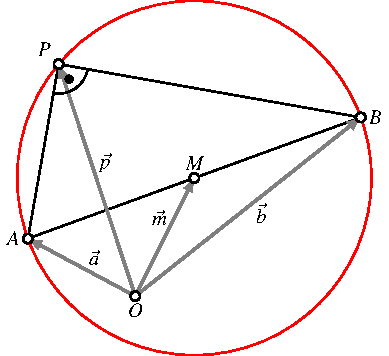
\includegraphics{4/images/thales.pdf}
\caption{Die Punkte $P$, von denen aus die Strecke $AB$ unter einem
rechten Winkel erscheint, bilden den Thaleskreis.
\label{thales-graphik}}
\end{figure}
Mit dem Skalarprodukt kann man ausdrücken, von welchen Punkten aus
eine Strecke $AB$ unter einem rechten Winkel gesehen wird, es ist
dies die Menge der Punkte $P$ mit der Eigenschaft
\[
\overrightarrow{AP}\cdot\overrightarrow{BP}=0
\]
(Abbildung~\ref{thales-graphik}).
Unter Verwendung der Konvention, dass kleine Buchstaben für die
Ortsvektoren der Punkte mit entsprechenden Grossbuchstaben stehen, ist
dies gleichbedeutend mit
\[
(\vec p-\vec a)\cdot(\vec p-\vec b)=0
\]
Ausmultiplizieren und quadratisch ergänzen ergibt
\begin{align*}
\vec p^2-\vec p\cdot\vec b-\vec a\cdot\vec p+\vec a\cdot\vec b&=0
\\
\vec p^2-(\vec a+\vec b)\cdot \vec p+\vec a\cdot\vec b&=0
\\
\vec p^2-2\left(\frac{\vec a+\vec b}{2}\right)\cdot \vec p
+\left(\frac{\vec a+\vec b}{2}\right)^2
-\left(\frac{\vec a+\vec b}{2}\right)^2
+\vec a\cdot\vec b&=0
\\
\left(\vec p
-\frac{\vec a+\vec b}{2}\right)^2&=
\left(\frac{\vec a+\vec b}{2}\right)^2-\vec a\cdot \vec b
\\
&=
\frac{\vec a^2+2\vec a\cdot\vec b+\vec b^2-4\vec a\cdot \vec b}{4}
\\
&=
\frac{\vec a^2-2\vec a\cdot\vec b+\vec b^2}{4}
\\
\left(\vec p
-\frac{\vec a+\vec b}{2}\right)^2&=
\left(\frac{\vec a-\vec b}{2}\right)^2
\end{align*}
Diese Gleichung beschreibt einen Kreis um den Punkt $(\vec a+\vec b)/2$
mit dem Radius $|\vec a-\vec b|/2$.
Dies ist der Thaleskreis.

%
% Tangente in einem Punkt
%
\subsection{Tangente oder Tangentialebene in einem Punkt}
\begin{figure}
\centering
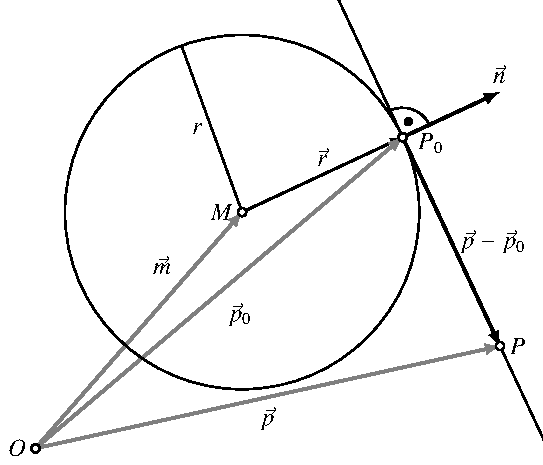
\includegraphics{4/images/tangente.pdf}
\caption{Tangente im Punkt $P_0$ an den Kreis um $M$ mit Radius $r$.
Der Vektor $\vec{p}-\vec{p}_0$ muss auf dem
Normalenvektor $\vec{n}$ senkrecht stehen, letzterer hat die Richtung
von $
%\overrightarrow{MP_0}=
\vec{p}_0-\vec{m}$.
\label{tangente-graphik}}
\end{figure}
Die Normale auf einen Kreis ist immer parallel zum Radiusvektor
(Abbildung~\ref{tangente-graphik}),
dasselbe gilt für eine Kugel.
Daher kann
man die Gleichung der Tangente in einem Punkt $P_0$ an einen Kreis
oder der Tangentialebene in einem Punkt der Kugel sofort angeben:
\begin{satz}\label{kugeltangentialebene}
Die Tangentialebene an eine Kugel mit Mittelpunktsortsvektor
$\vec m$ und Radius  $r$ im Punkt mit Ortsektor $\vec p_0$ ist
\begin{equation}
\{\vec p\;|\;
(\vec p-\vec p_0)\cdot(\vec p_0-\vec m)=0
\}
\label{eqn-kugeltangente}
\end{equation}
\end{satz}
Diese Form (\ref{eqn-kugeltangente}) ist noch nicht optimal, man kann den
Radius nicht direkt ablesen.
Addieren wir jedoch noch die Gleichung
der Kugel für den Vektor $\vec p_0$, erhalten wir
\begin{align*}
(\vec p-\vec p_0)\cdot(\vec p_0-\vec m)&=0\\
(\vec p_0-\vec m)\cdot(\vec p_0-\vec m)&=r^2\\
\Rightarrow\qquad
(\vec p-\vec m)\cdot(\vec p_0-\vec m)&=r^2
\end{align*}
Die Tantentengleichung ist also die Kreisgleichung, in der man
eine Kopie von $\vec p$ durch den Berührpunkt $\vec p_0$ ersetzt
hat.

%
% Tangente/Tangentialebene von einem Punkt aus
%
\subsection{Tangente von einem Punkt an einen Kreis}
Es sind die Gleichungen der Tangenten an einen Kreis $K(M,r)$ zu finden,
welche durch den Punkt $P$ gehen.
Die klassische Konstruktion der
Elementargeometrie verlangt, dass über der Strecke $MP$ der
Thaleskreis gezeichnet wird, die Schnittpunkte des Thaleskreis mit
$K(M,r)$ sind die Berührpunkte der Tangenten.

Die Tangenten sollen jetzt aber auf rein algebraische Art gefunden
werden.
Das Problem wäre im wesentlich gelöst, wenn der Berührpunkt $P_0$
mit Ortsvektor
$\vec p_0$ bekannt wäre.
Dieser muss natürlich auf dem Kreis liegen,
also
\[
(\vec p_0-\vec m)^2=r^2.
\]
Ausserdem muss der Punkt $P$ auf der Tangente im Punkt $P_0$ liegen,
also muss $MP_0$ senkrecht auf $PP_0$ stehen:
\begin{equation}
(\vec p_0-\vec m)\cdot(\vec p-\vec p_0)=0
\label{thalesbedingung}
\end{equation}
Damit haben wir zwei Gleichungen für die beiden unbekannten Koordinaten
von $P_0$ gefunden, im Allgemeinen werden sie die Bestimmung von $\vec p_0$
ermöglichen (Ausnahmen: $P$ im Inneren des Kreises).

Zur Lösung multiplizieren wir die zweite Gleichung noch aus
\begin{align*}
\vec p_0^2-\vec m\cdot\vec p_0-\vec p\cdot\vec p_0+\vec m\cdot\vec p&=0
\\
\vec p_0^2-\vec p_0\cdot (\vec m+\vec p)+\vec m\cdot\vec p&=0
\\
\vec p_0^2-2\vec p_0\cdot \left(\frac{\vec m+\vec p}{2}\right)+\vec m\cdot\vec p&=0
\\
\vec p_0^2-2\vec p_0\cdot \left(\frac{\vec m+\vec p}{2}\right)+
\left(\frac{\vec m+\vec p}2\right)^2
-\left(\frac{\vec m+\vec p}2\right)^2
+\vec m\cdot\vec p&=0
\\
\left(\vec p_0- \frac{\vec m+\vec p}{2}\right)^2
&=
\left(\frac{\vec m+\vec p}2\right)^2
-\vec m\cdot\vec p
\\
\left(\vec p_0- \frac{\vec m+\vec p}{2}\right)^2
&=
\left(\frac{\vec m-\vec p}2\right)^2
\end{align*}
Dies ist wieder ein Kreis mit Mittelpunkt $(\vec m+\vec p)/2$ und
Radius $|\vec m-\vec p|/2$, also wieder ein Thaleskreis.
Das ist natürlich nicht überraschend, die Bedingung (\ref{thalesbedingung})
ist ja nichts anderes als die Definition des Thaleskreises.
Die algebraische Rechnung macht also nichts anderes als die klassische
Konstruktion.

%
%  Reflexion eines Lichtstrahls und Ray-Tracing
%
\subsection{Reflexion eines Lichtstrahls}
\begin{figure}
\begin{center}
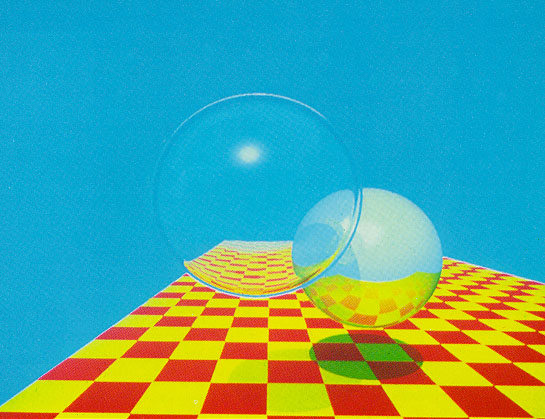
\includegraphics[width=1\hsize]{graphics/raytracing}
\end{center}
\caption{Mit Ray Tracing erzeugtes computergeneriertes Bild\label{raytracing}}
\end{figure}
Computergraphik-Effekte sind aus modernen Filmen nicht mehr wegzudenken.
Ganze Spielfilme wurden schon vollständig im Computer erzeugt.
Wie können die Bilder so realistisch wirken?

In Abschnitt \ref{spiegelung} haben wir gelernt, wie ein Vektor
gespiegelt wird.
Wir können also den Lichtstrahl, der in das Auge
des Beobachters einer Szene fällt, zurückverfolgen und seine Reflektion
an jeder beliebigen reflektierenden Fläche der Szene berechnen, bis wir bei
einer Lichtquelle oder einem nicht reflektierenden Objekt ankommen.
Die an diesem Punkt abgestrahlte Farbe ist dan jene, die der Beobachter
wahrnimmt.
Dieses Verfahren nennt man Ray Tracing.
Offenbar ist es sehr
aufwendig, denn Lichtstrahlen können nicht nur reflektiert, sondern auch
gestreut werden, und sie können zum Beispiel durch Nebel abgeschwächt
werden.
Die Berechnung hochauflösender Szenen ist daher sehr aufwendig,
die Herstellung von CG-Filmen in Spielfilm-Länge, wie Pixar sie beispielsweise
produziert, benötigt die Rechenleistung grosser Computer-Cluster.

Die Berechnung der Reflexion an einer Kugel wie in Abbildung \ref{raytracing}
erfolgt nach folgendem Algorithmus:
\begin{enumerate}
\item Berechne den Durchstosspunkt des Lichtstrahles mit der reflektierenden
Kugeloberfläche wie in \ref{durchstosspunktkugel} beschrieben.
\item Berechnet die Normale im Durchstosspunkt gemäss Satz \ref{kugeltangentialebene}.
\item Berechne die gespiegelte Gerade gemäss Abschnitt \ref{spiegelung}.
\end{enumerate}
Dieses Verfahren wird jedoch nicht nur für die Computergraphik verwendet,
sondern auch in der Optik.
Spiegelteleskope bestehen aus gekrümmten Spiegeln,
durch Berechnung der Strahlen kann man erfahren, welche Abbildungsqualität
man von dem Teleskop erwarten kann.


%
% abbildungen.tex
%
% (c) 2018 Prof Dr Andreas Müller, Hochschule Rapperswil
% 
\section{Orientierungserhaltende Abbildungen}
\rhead{Orientierungserhaltende Abbildungen}
Wie im Falle des Skalarproduktes bilden die Abbildungen, die den Flächeninhalt,
das Volumen und/oder die Orientierung erhalten, eine Gruppe.

\subsection{Determinante und Fläche}
Sei $A$ eine Abbildungsmatrix in einem zweidimensionalen Raum.
Die Spalten von $A$ sind die Bilder der Standardbasisvektoren.
Die Determinante von $A$ ist der orientierte Flächeninhalt des Parallelogramms 
aufgespannt von den beiden Spaltenvektoren.
Die von $A$ beschriebene Abbildung macht also aus einem Quadrat mit
orientiertem Flächeninhalt $F$
eine Parallelogramm mit orientierten Flächeninhalt $\det(A)\cdot F$.

Der Flächeninhalt eines Gebietes in der Ebene bleibt unter der Abbildung
$A$ genau dann erhalten, wenn $\det(A)=\pm 1$ gilt.
Falls $\det(A)=-1$ ändert die Orientierung.
Eine Abbildung, die nicht nur den Flächeninhalt, sondern auch die
Orientierung erhält, erfüllt $\det(A)=1$.

Eine Abbildung mit $\det(A)=1$ muss nicht orthogonal sein, wie das Beispiel
\begin{align*}
A
&=
\begin{pmatrix}2&3\\1&2\end{pmatrix}
\qquad\Rightarrow\qquad
\det(A) = 2\cdot 2-3\cdot 1 =1
\\
A^tA
&=
\begin{pmatrix}2&1\\3&2\end{pmatrix}
\begin{pmatrix}2&3\\1&2\end{pmatrix}
=
\begin{pmatrix}
5&7\\
7&13
\end{pmatrix}
\ne
\begin{pmatrix}
1&0\\
0&1
\end{pmatrix}.
\end{align*}
Ausserdem müsste eine orthogonale Matrix Spaltenvektoren der Länge $1$ haben,
während die Spalten von $A$ ganz offensichtlich länger als $1$ sind.

\subsection{Determinante und Volumen}
Aus dem gleichen Argument wie beim Flächeninhalt folgt, dass eine
Abbildungsmatrix $A$ in einem dreidimensionalen Raum einen Körper mit
Volumen $V$ auf einen Körper mit Volumen $\det(A)\cdot V$.
Eine Abbildung $A$ erhält das Volumen, wenn $\det(A)=\pm 1$,
die Orientierung bleibt ebenfalls erhalten, wenn $\det(A)=1$.

\subsection{Spezielle lineare und orthogonale Gruppe}
Die orientientierungserhaltenden Abbildungen bilden die Teilmenge
\[
\operatorname{SL}_n(\mathbb R)
=
\{
A\in M_n(\mathbb R)
\;|\;
\det(A) = 1
\}.
\]
Für $A,B\in\operatorname{SL}_n(\mathbb R)$ lässt die
Produktformel
\[
\det(AB)=\det(A)\det(B) = 1
\]
die Schlussfolgerung zu, dass auch $AB\in\operatorname{SL}_n(\mathbb R)$.
Die Menge $\operatorname{SL}_n(\mathbb R)$ ist daher eine Gruppe, sie
heisst die {\em spezielle lineare Gruppe}.

Abbildungen $A$, die das Skalarprodukt erhalten, sind in $\operatorname{O}(n)$ und erfüllen
\[
A^tA=E
\quad\Rightarrow\quad
1
=
\det(E)
=
\det(A^tA)=\det(A^t)\det(A)=\det(A)^2
\quad\Rightarrow\quad
\det(A) = \pm 1.
\]
Die Abbildungen, die sowohl das Skalarprodukt als auch die Orientierung
erhalten, zeichnen sich also dadurch aus, dass sie sowohl in
$\operatorname{O}(n)$ als auch in $\operatorname{SL}_n(\mathbb R)$ sein, wir nennen diese
Gruppe
\[
\operatorname{SO}(n) 
=
\operatorname{O}(n) \cap \operatorname{SL}_n(\mathbb R)
=
\{
A\in M_n(\mathbb R)\;|\; A^tA=E\wedge \det(A) = 1
\}
\]
die spezielle orthogonale Gruppe.
Dies sind die Bewegungen, die den Nullpunkt unverändert lassen,
Längen und Winkel erhalten und die Orientierung nicht ändern.
Dies sind genau die Drehmatrizen.
Die Determinante ist also das in Abschnitt~\ref{subsection:orthogonale gruppe}
angekündigte Kriterium, mit welchem wir Drehmatrizen von Matrizen
unterscheiden können, die eine Spiegelungskomponente enhalten.

Die Differenz $\operatorname{O}(n) \setminus \operatorname{SO}(n)$
besteht aus Matrizen, die zwar das Skalarprodukt erhalten, aber die
Orientierung umkehren.
Ist $S_x$ die Spiegelung an der Ebene senkrecht zur $x$-Achse und ist
$A\in \operatorname{O}(n) \setminus \operatorname{SO}(n)$, dann ist
\[
\det(S_xA)= \det(S_x)\det(A) = (-1)\cdot(-1)=1
\qquad\Rightarrow\qquad
S_xA\in\operatorname{SO}(n).
\]
Dies bedeutet, dass die Multiplikation mit $S_x$ eine bijektive Abbildung
\[
\operatorname{SO}(n) \to \operatorname{O}(n)\setminus\operatorname{SO}(n)
:
A\mapsto S_xA
\]
definiert.
Die Gruppe $\operatorname{O}(n)$ besteht also aus zwei gleichartig gebauten
Teilmengen, $\operatorname{SO}(n)$  und
$\operatorname{O}(n)\setminus\operatorname{SO}(n)$.




%
% ueberbestimmt.tex
%
% (c) 2018 Prof Dr Andreas Müller, Hochschule Rapperswil
%
\section{Überbestimmte Gleichungssysteme -- ``Least Squares''%
\label{section:ueberbestimmt}}
\index{Gleichungssystem!überbestimmtes}
Bei einem überbestimmten Gleichungssystem, also einem Gleichungssystem
mit mehr Gleichungen als Unbekannten, kann man im Allgemeinen nicht davon
ausgehen, dass es überhaupt eine Lösung gibt.
Ein solches Gleichungssystem hat die Form
\[
A v= b,
\]
wobei $A$ eine Matrix ist, die mehr Zeilen als Spalten hat.

Betrachten wir als Beispiel das Gleichungssystem
\[
\begin{pmatrix}
 6&14\\
12&28\\
 9&21
\end{pmatrix}
\begin{pmatrix}v_1\\v_2\end{pmatrix}
=
\begin{pmatrix}2\\4\\4\end{pmatrix}.
\]
Die Bildmenge der Abbildungsmatrix $A$ beschreibt eine Ebene durch
den Nullpunkt mit den Parametern $v_1$ und $v_2$.
Das Gleichungssystem sucht also nach den Parametern $v_1$ und $v_2$
des Punktes auf der Ebene mit den Koordinaten $(2,4,4)$.
Solche Parameterwerte müssen aber gar nicht existieren, es ist
ja nicht klar, dass der Punkt überhaupt auf der Ebene liegt.

Das Beispiel zeigt aber noch eine weitere Schwierigkeit.
Die beiden Spaltenvektoren von $A$ sind nämlich linear abhängig,
die zweite Spalte ist das $\frac{7}{3}$-fache der ersten Spalte.
Der Rang der Matrix ist daher $1$, die Bildmenge ist sogar nur
eine Gerade.
Man erkennt zum Beispiel, dass der Punkt $(2,4,3)$ auf der Geraden
liegt.
Der gegebene Punkt $(2,4,4)$ kann aber nicht auf der Geraden liegen.
Das Gleichungssystem ist nicht lösbar.

\rhead{Überbestimmte Gleichungssysteme}
%
% Lösungen im Sinne des kleinsten Abstandes
%
\subsection{Lösung im Sinne des kleinsten Abstandes}
Das beste, was man erwarten kann, ist ein Vektor $v_0$ so, dass
der Abstand des Punktes $ b$ von der Ebene (Gerade) bestehend
aus allen $Av$ für $v=v_0$ am kleinsten wird.
Dies geschieht natürlich genau dann, wenn der Differenzvektor $b-Av_0$ auf
allen Vektoren von $Av$ senkrecht steht.

Die Menge der Vektoren der Form $Av$ wird von den Spalten von $A$
aufgespannt.
Es genügt also zu testen, ob $b-Av_0$ auf diesen
Vektoren senkrecht steht.
Dazu müssen die Skalarprodukte von
Spalten von $A$ mit dem Vektor $b-Av_0$ verschwinden, oder
\[
A^t(b-Av_0)=0
\quad
\Rightarrow
\quad
A^tAv_0=A^tb
\]
wir haben also ein Gleichungssystem gefunden mit Matrix $A^tA$ und
rechter Seite $A^tb$, welches als Lösung den gesuchten Vektor
$v_0$ hat.
$A^t$ hat so viele Zeilen wie $v$ Komponenten hat, also
handelt es sich um ein Gleichungssystem mit gleich vielen Gleichungen
wie Unbekannten.
Es wird im Allgemeinen eine eindeutig bestimmte Lösung haben.

\begin{satz} Sei $A$ eine $n\times m$ Matrix und $b$ ein $n$-dimensionaler
Vektor.
Eine Lösung im Sinne minimaler quadrierter Abstände
$
(Av-b)\cdot(Av-b)
$
ist Lösung des Gleichungssystems
\[
A^tAv=A^tb
\]
mit $m$ Gleichungen und $m$ Unbekannten.
\end{satz}

\begin{beispiel}
Man finden den Fusspunkt des Lotes vom Punkt $P=(9,10,7)$ auf die Ebene
durch $O$, $A=(8,10,10)$ und $B=(9,13,12)$.

Der Fusspunkt des Lotes ist der Punkt der Ebene, der den geringsten
Abstand zu $P$ hat.
Die Ebenengleichung ist
\[
A\begin{pmatrix}s\\t\end{pmatrix}=
\begin{pmatrix}
 8& 9\\
10&13\\
10&12
\end{pmatrix}
\begin{pmatrix}s\\t\end{pmatrix}.
\]
Gesucht wird die ``beste Lösung'' von
\[
A\begin{pmatrix}s\\t\end{pmatrix}=\begin{pmatrix}9\\10\\7\end{pmatrix}=b
\]
Dazu muss zunächst die Matrix $A^tA$ und der Vektor $A^tb$
berechnet werden.
\[
A^tA=\begin{pmatrix}
264&322\\
322&394
\end{pmatrix}
,\qquad
A^tb=\begin{pmatrix}
242\\295
\end{pmatrix}.
\]
Daraus findet man die Lösung für $s$ und $t$ numerisch zu
\[
\begin{pmatrix}s\\t \end{pmatrix}
=
\begin{pmatrix}
   1.07831\\
  -0.13253
\end{pmatrix}
\]
und durch Einsetzen in die Ebenengleichung den Ortsvektor des Fusspunktes
\[
\vec f = \begin{pmatrix}
   7.4337\\
   9.0602\\
   9.1928
\end{pmatrix}.
\]
Man kann dieses Resultat dadurch kontrollieren, dass man nachrechnet, ob
$\vec p-\vec f$ senkrecht auf beiden Richtungsvektoren der Ebene
steht:
\[
(\vec p-\vec f)^tA=\begin{pmatrix}
  -1.7451\cdot10^{-11}&  -2.1316\cdot 10^{-11}
\end{pmatrix},
\]
im Rahmen der Rechengenauigkeit steht die Differenz also tatsächlich auf
den Richtungsvektoren senkrecht.
\end{beispiel}

%
% Alles in einem Schritt
%
\subsection{``Alles in einem Schritt''}
In Kapitel~\ref{chapter:affin} wurde gezeigt, wie man Probleme der
affinen Geometrie mit nur einer Durchführung des Gauss-Algorithmus
lösen konnte.
Bei der soeben vorgestellten Lösung des Fusspunkt-Problems
musste man aber wieder in mehrere Schritten vorgehen.
Zuerst wurden $s$ und $t$ bestimmt,
erst in einem zweiten Schritt konnte der Fusspunkt des Lotes
berechnet werden.

Natürlich ist das auch für dieses Problem möglich, man behandelt
$x$, $y$ und $z$ einfach als zusätzliche Variablen, die als Koordinaten
von $Av$ berechnet werden.
Das Gauss-Tableau dazu ist
\[
\begin{tabular}{|>{$}c<{$}>{$}c<{$}>{$}c<{$}>{$}c<{$}|>{$}c<{$}|}
\hline
x&y&z&s\quad t&\\
\hline
1&0&0&        &0\\
0&1&0&-A   &0\\
0&0&1&        &0\\
\hline
 & & &A^tA    &A^tb\\
\hline
\end{tabular}
\]
\begin{beispiel}
Für das Zahlenbeispiel lautet dieses Gauss-Tableau:
\[
\begin{tabular}{|>{$}c<{$}>{$}c<{$}>{$}c<{$}>{$}c<{$}>{$}c<{$}|>{$}c<{$}|}
\hline
x&y&z&s  &  t&\\
\hline
1&0&0& -8& -9&0\\
0&1&0&-10&-13&0\\
0&0&1&-10&-12&0\\
\hline
0&0&0&264&322&242\\
0&0&0&322&394&295\\
\hline
\end{tabular}
\rightarrow
\begin{tabular}{|>{$}c<{$}>{$}c<{$}>{$}c<{$}>{$}c<{$}>{$}c<{$}|>{$}r<{$}|}
\hline
x&y&z&s  &  t&\\
\hline
1&0&0&0&0&7.4337\\
0&1&0&0&0&9.0602\\
0&0&1&0&0&9.1928\\
\hline
0&0&0&1&0&1.0783\\
0&0&0&0&1&-0.1325\\
\hline
\end{tabular}
\]
Man erhält also genau die bereits früher gefundenen Lösungen.
\end{beispiel}

%
% Der allgemein Fall
%
\subsection{Der allgemeine Fall}
Überbestimmte Gleichungssysteme sind Gleichungssysteme der Form
$Ax=b$ mit einer $m\times n$-Matrix mit $m>n$, also mehr Gleichungen
als Unbekannten.
Im Allgemeinen sind sie nicht lösbar, weil $b$ nicht
im Bild von $A$ enthalten ist: $b\not\in \operatorname{im}A$.

Statt einer exakten Lösung könnte man daher eine approximative
Lösung suchen, welche die Gleichung möglichst gut erfüllt.
Der Vektor $Ax-b$ sollte also möglichst kurz sein.
Geometrisch
geht es also darum, das Lot vom Punkt $b$ auf den von den Spaltenvektoren
von $A$ aufgespannten Unterraum zu fällen.
Wir suchen also
einen Vektor, der auf allen Spaltenvektoren von $A$ senkrecht steht.
Das Skalarprodukt von Spaltenvektoren von $A$ mit $Ax-b$ ist aber
$A^t(Ax-b)$, wir müssen also das Gleichungssystem
\[A^t(Ax-b)=0\]
lösen.
Nach Ausmultiplizieren bekommen wir
\begin{equation}
A^tAx-A^tb=0\quad\Rightarrow\quad A^tAx=A^tb\quad\Rightarrow\quad
x=(A^tA)^{-1}A^tb.
\label{uberbestimmt}
\end{equation}
Man beachte, dass $A$ nicht quadratisch ist, und dass man daher
nicht mit $(A^tA)^{-1}A^t=A^{-1}(A^t)^{-1}A^t=A^{-1}$ vereinfachen
kann.

\begin{beispiel}
Sei 
\[
A=\begin{pmatrix}1\\1\\1\\\end{pmatrix},\quad b=\begin{pmatrix}1\\2\\3\end{pmatrix}.
\]
Offenbar ist $b\not\in\operatorname{im}A$.
Nach der Formel (\ref{uberbestimmt}) muss man zunächst $A^tA$ ausrechnen:
\[
A^tA=\begin{pmatrix}1&1&1\end{pmatrix}\begin{pmatrix}1\\1\\1\end{pmatrix}=3.
\]
Damit kann man jetzt nach (\ref{uberbestimmt}) die bestmögliche
approximative Lösung finden:
\[
x=\frac13\cdot\begin{pmatrix}1&1&1\end{pmatrix}
\begin{pmatrix}1\\2\\3\end{pmatrix}=2.
\]
Der von $b$ am wenigsten weit entfernte Punkt der Geraden mit
Richtung $A$ ist also der Punkt $(2,2,2)$.
\end{beispiel}

%
% Anwendungen der Methode der kleinsten Quadrate
%
\subsection{Anwendungen der Methode der kleinsten Quadrate}
Die Bedeutung der Methode der kleinsten Qudarate besteht darin, dass 
man in der Praxis sehr oft die Situation hat, dass man deutlich mehr
Daten hat als nötig, um die Parameter eines Problems zu bestimmen.
Zum Beispiel genügt es, drei Punkte eines Kreises zu kennen, um
Mittelpunkt und Radius exakt bestimmen zu können.
Oder zwei Punkte bestimmen eine Gerade eindeutig.
In der Praxis misst man meistens mehr Punkte.
Allerdings sind die Messungen mit Messfehlern behaftet.
Die Methode der kleinsten Quadrate erlaubt dann, die bestmöglichen
Werte für die Parameter zu finden.
Dies soll an zwei Beispielen illustriert werden.

\subsubsection{Gerade durch Punkte}
\begin{figure}
\centering
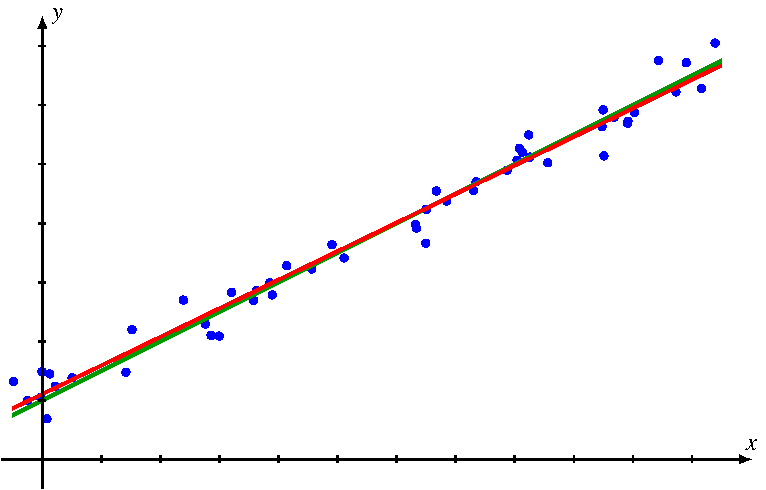
\includegraphics{4/images/linreg.pdf}
\caption{Bestimmung einer Geraden, die eine Menge von Punkten am besten
approximiert.
Die blauen Punkte sind entstanden, indem Punkte der grünen Gerade
mit einer zufälligen Abweichungen gestört wurden.
Die rot eingezeichnete Regeressionsgerade approximiert die ursprüngliche
Gerade mit grosser Genauigkeit.
\label{skript:linreg-abb}}
\end{figure}
Gegeben sind Punkte $(x_i,y_i)$ mit $1\le i\le n$, die ungefähr auf
einer Geraden $y={\color{red}a}x+{\color{red}b}$ liegen.
Gesucht sind die Werte von $\color{red}a$ und $\color{red}b$
(Abbildung~\ref{skript:linreg-abb}).
Zur Verdeutlichung heben wir im
Folgenden die Unbekannten rot hervor.
Wären die Punkte exakt auf der Geraden, müsste jeder die Geradengleichung
erfüllen, wir erhielten also die Gleichungen
\begin{equation}
\begin{linsys}{2}
{\color{red}a}x_1&+     &{\color{red}b}&=&y_1\\
{\color{red}a}x_2&+     &{\color{red}b}&=&y_2\\
                 &\vdots&              & &\vdots\hspace*{1mm}\\
{\color{red}a}x_n&+     &{\color{red}b}&=&y_n
\end{linsys}
\label{leastsquares:gerade}
\end{equation}
Dies ist ein Gleichungssystem für die Unbekannten ${\color{red}a}$ und
${\color{red}b}$ mit $n$
Gleichungen, im Allgemeinen ist es also überbestimmt.

Die Gleichung \eqref{leastsquares:gerade} kann mit dem Standardverfahren
gelöst werden.
Dazu schreiben wir zunächst die Matrix $A$ und den Vektor $b$ auf:
\[
A
=
\begin{pmatrix}
x_1   &1     \\
x_2   &1     \\
\vdots&\vdots\\
x_n   &1
\end{pmatrix}
,\qquad
x=
\begin{pmatrix}
\color{red}a\\
\color{red}b
\end{pmatrix},
\qquad
b
=
\begin{pmatrix}
y_1\\
y_2\\
\vdots\\
y_n
\end{pmatrix}
\]
Für die Lösung müssen wir $A^tA$ und $A^tb$ berechnen:
\begin{align*}
A^tA
&=
\begin{pmatrix}
x_1&x_2&\dots&x_n\\
 1 & 1 &\dots& 1
\end{pmatrix}
\begin{pmatrix}
x_1   &1     \\
x_2   &1     \\
\vdots&\vdots\\
x_n   &1
\end{pmatrix}
=
\begin{pmatrix}
\displaystyle\sum_{i=1}^n x_i^2 & \displaystyle\sum_{i=1}^n x_i \\
\displaystyle\sum_{i=1}^n x_i   &       n
\end{pmatrix}
\\
A^tb
&=
\begin{pmatrix}
x_1&x_2&\dots&x_n\\
 1 & 1 &\dots& 1
\end{pmatrix}
\begin{pmatrix}
y_1\\
y_2\\
\vdots\\
y_n
\end{pmatrix}
=
\begin{pmatrix}
\displaystyle \sum_{i=1}^n x_iy_i\\
\displaystyle \sum_{i=1}^n y_i
\end{pmatrix}.
\end{align*}
Die Determinante von $A^tA$ ist
\[
\det(A^tA)
=
n\sum_{i=1}^n x_i^2 -\biggl(\sum_{i=1}^n x_i\biggr)^2
.
\]
Dieses Gleichungssystem kann man jetzt mit der Cramerschen Regel für die
Unbekannte ${\color{red}a}$ lösen:
\begin{align*}
{\color{red}a}
&=
\frac{\displaystyle
n\sum_{i=1}^n x_iy_i-\sum_{i=1}^nx_i\sum_{i=1}^ny_i
}{\displaystyle
n\sum_{i=1}^n x_i^2 -\biggl(\sum_{i=1}^n x_i\biggr)^2
}
=
\frac{\displaystyle
\frac1n\sum_{i=1}^n x_iy_i-\frac1n\sum_{i=1}^nx_i\cdot \frac1n\sum_{i=1}^ny_i
}{\displaystyle
\frac1n\sum_{i=1}^n x_i^2 -\biggl(\frac1n\sum_{i=1}^n x_i\biggr)^2
}.
\end{align*}
Den Achsenabschnitt $\color{red}b$ könnte man natürlich auch so finden,
es geht aber auch direkter.
Bildet man die Summe der Gleichungen 
\ref{leastsquares:gerade}, erhält man
\[
{\color{red}a}
\sum_{i=1}^n x_i
+
n{\color{red}b}
=
\sum_{i=1}^n y_i.
\]
Auflösen nach $\color{red}b$ ergibt
\begin{align*}
{\color{red}b}
&=
\frac1n\sum_{i=1}^n y_i
-{\color{red}a}
\cdot
\frac1n\sum_{i=1}^n x_i.
\end{align*}
Die so gefundene Gerade  mit der Gleichung
$y={\color{red}a}x+{\color{red}b}$
heisst auch {\em Regressionsgerade}.
\index{Regressionsgerade}

\subsubsection{Kreis durch Punkte}
\begin{figure}
\centering
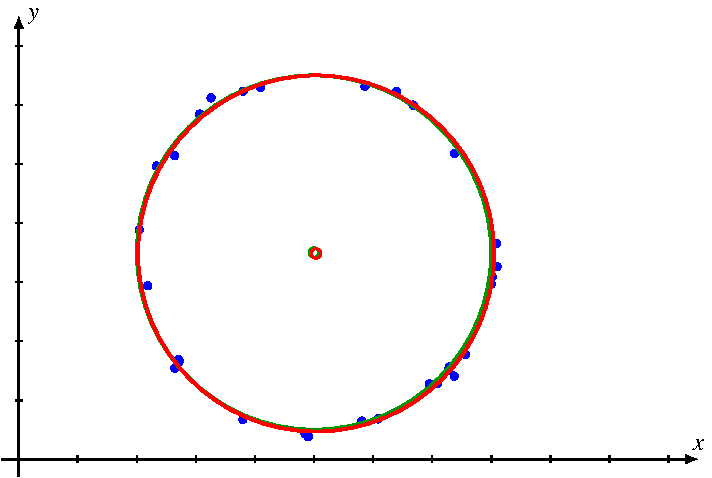
\includegraphics{4/images/kreis.pdf}
\caption{Bestimmung eines Kreises, der eine Menge von Punkten am besten
approximiert.
Die blauen Punkte sind entstanden, indem Punkte des grünen Kreises
mit einer zufälligen Abweichungen gestört wurden.
Der rot eingezeichnete Kreis approximiert den ursprünglichen
Kreis mit grosser Genauigkeit.
\label{skript:linreg-abb}}
\end{figure}
Gegeben sind die Punkte $(x_i,y_i)$ mit $1\le i\le n$, die ungefähr
auf einem Kreis liegen.
Gesucht sind Mittelpunkt $M=(m_x,m_y)$ und Radius $r$ dieses Kreises.
Wieder heben wir zur Verdeutlichung im Folgenden die Unbekannten farbig
hervor.
Zunächst müssen wir Gleichungen für die gesuchten Variablen aufstellen.
Die Gleichung eines Kreises ist
\[
(x_i - {\color{red}m_x})^2 + (y_i - {\color{red}m_y})^2 = {\color{red}r}^2.
\]
Diese Gleichungen sind allerdings nicht linear.
Das Standardverfahren ist also nicht anwendbar.
Wir multiplizieren daher aus, und erhalten
\[
x_i^2 - 2x_i {\color{red}m_x} + {\color{red}m_x}^2
+
y_i^2 - 2y_i {\color{red}m_y} + {\color{red}m_y}^2
=
{\color{red}r}^2.
\]
Indem wir die Quadrate der Variablen zu einer neuen Variable 
\[
{\color{red}c}
=
{\color{red}r}^2
-
{\color{red}m_x}^2
-
{\color{red}m_y}^2
\]
zusammenfassen, können wir die Gleichungen in lineare Form bringen:
\begin{equation}
2x_i{\color{red}m_x}
+
2y_i{\color{red}m_y}
+
{\color{red}c}
=
x_i^2+y_i^2,\qquad 1\le i\le n.
\end{equation}
In dieser Form lässt sich das Standardverfahren anwenden, die Matrix
$A$ und die Vektoren $x$ und $b$ sind
\begin{align*}
A
&=
\begin{pmatrix}
2x_1  & 2y_1 & 1    \\
2x_2  & 2y_2 & 1    \\
\vdots&\vdots&\vdots\\
2x_n  & 2y_n & 1    \\
\end{pmatrix},
&
x&=\begin{pmatrix}
{\color{red}m_x}\\
{\color{red}m_y}\\
{\color{red}c}
\end{pmatrix}
&&\text{und}&
b
&=
\begin{pmatrix}
x_1^2+y_1^2\\
x_2^2+y_2^2\\
\vdots\\
x_n^2+y_n^2
\end{pmatrix}.
\end{align*}
Aus der Lösung kann dann der Radius als 
\[
{\color{red}r}= 
\sqrt{
{\color{red}c}
+
{\color{red}m_x}^2
+
{\color{red}m_y}^2
}
\]
bestimmt werden.
Abbildung~\ref{skript:linreg-abb} zeigt, wie der Kreis mit grosser
Genauigkeit auch aus stark fehlerbehafteten Punkten bestimmt werden
kann.

\subsubsection{Drehung und Translation finden}
\begin{figure}
\centering
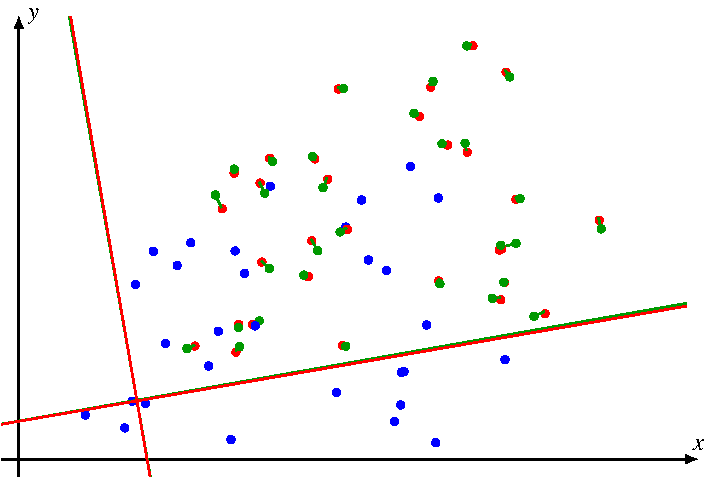
\includegraphics{4/images/bewegung.pdf}
\caption{Bestimmung von Drehwinkel und Translation einer Bewegung.
Die ursprüngliche Bewegung bewegt das schwarze Koordinatenkreuz auf
die grünen Achsen.
Die blauen Punkte werden mit dieser Bewegung abgebildet aber zusätzlich
noch mit einem zufälligen Fehler überlagert, so entstehen die grünen Punkte.
Die kurzen grünen Linien beginnen beim exakten Bild eines blauen Punktes.
Das im Text beschriebene Verfahren liefert den Drehwinkel und die
Verschiebung, die das Koordinatensystem auf die roten Achsen bewegt.
Damit werden die blauen Punkte auf die roten Punkte abgebildet.
Es zeigt sich, dass die grünen Linien ziemlich genau dort beginnen, wo
die gefundene Bewegung die blauen Punkte hinbewegt, das Verfahren kann
sowohl die Bewegung als auch die Fehler (die grünen Linien)
recht genau ermitteln.
\label{skript:bewegung-leastsquares}}
\end{figure}
Das Regstrierungsproblem in der Bildverarbeitung verlangt, zwei Bilder
der gleichen Szene mit Hilfe einer Drehung und Translation zur Deckung
zu bringen.
In der Astrophotographie kann man zum Beispiel in zwei Bildern die
Positionen der
Sterne $(x_i,y_i)$ und $(x_i',y_i')$ in jedem Bild finden und dann
die Transformation suchen, die die Punkte möglichst genau zur Deckung bringt.
Diese Transformation kann in Matrixform als
\begin{align*}
\begin{pmatrix}
x_i'\\y_i'
\end{pmatrix}
=
\begin{pmatrix}
\cos{\color{red}\alpha}&-\sin{\color{red}\alpha}& \color{red}t_x\\
\sin{\color{red}\alpha}&\phantom{-} \cos{\color{red}\alpha}& \color{red}t_y
\end{pmatrix}
\begin{pmatrix}
x_i\\y_i\\1
\end{pmatrix}
\end{align*}
geschrieben werden.
Der Winkel ${\color{red}\alpha}$ tritt in den Gleichungen nicht
linear auf.
Stattdessen verwenden wir
${\color{red}c}=\cos{\color{red}\alpha}$
und
${\color{red}s}=\sin{\color{red}\alpha}$
als Unbekannte.
Die Gleichungen werden 
\begin{equation}
\begin{linsys}{6}
x_i{\color{red}c} &-& y_i{\color{red}s} &+& {\color{red}t_x} & &                &=&x_i'\\
y_i{\color{red}c} &+& x_i{\color{red}s} & &                  &+&{\color{red}t_y}&=&y_i'\\
\end{linsys}
\end{equation}
Dies ist ein überbestimmtes lineares Gleichungssystem von
$2n$-Gleichungen für die vier Unbekannten
${\color{red}c}$,
${\color{red}s}$,
${\color{red}t_x}$ und
${\color{red}t_y}$.
Die Matrix $A$ und die Vektor $x$ und $b$ sind
\begin{align*}
A&=
\begin{pmatrix}
x_1&-y_1&1&0\\
y_1& x_1&0&1\\
x_2&-y_2&1&0\\
y_2& x_2&0&1\\
\vdots&\vdots&\vdots&\vdots\\
x_n&-y_n&1&0\\
y_n& x_n&0&1\\
\end{pmatrix},
&
x
&=
\begin{pmatrix}
{\color{red}c}\\
{\color{red}s}\\
{\color{red}t_x}\\
{\color{red}t_y}
\end{pmatrix}
&&\text{und}&
b
&=
\begin{pmatrix}
x_1'\\
y_1'\\
x_2'\\
y_2'\\
\vdots\\
x_n'\\
y_n'\\
\end{pmatrix}
\end{align*}
Es ist nicht garantiert, dass die Lösung
\[
\lambda^2
=
{\color{red}c}^2
+
{\color{red}s}^2
=1
\]
erfüllen wird, wie das für $\cos\alpha$ und $\sin\alpha$ der Fall wäre.
Die Bedeutung von $\lambda$ ist die eines zusätzlichen Streckungsfaktors,
dem das Bild für optimale Deckung auch noch unterworfen werden sollte.
Abbildung~\ref{skript:bewegung-leastsquares} zeigt an einem Beispiel, wie
das Verfahren die Bewegung aus wenigen Punkten ermitteln kann.




